\section{Theoretical Background}

% === HIPPOCAMPUS ===================================

\begin{frame}
\frametitle{Hippocampus}
	\begin{itemize}
		\item<1-> Has the shape of a seahorse
		\item<2-> Key factor in forming memories (not preserving them!)~\cite{Trepel17N}
		\item<3-> Related to emotions~\cite{GarzorzStark18BN}
		\item<4-> Responsible for any kind of navigation (e.g. ranking stuff like danger of animals)
		\begin{itemize}
			\item<5-> Crafts a cognitive room of the ``surroundings'' by using place cells and grid cells
			\item<6-> Place cell: irregular arranged, fires at specific positions in space (``states'') % [deutschlandfunk]
			\item<7-> Grid cell: lattice-like arranged, fires continuously
		\end{itemize}
	\end{itemize}
% --- BILDER -----------------------------------
\begin{columns}
    % SPALTE 1, Hippocampus und Seepferdchen
    \begin{column}{0.3\textwidth}
        \vspace*{-2mm}
        \begin{figure}
            \centering
                \includegraphics<1->[width=\columnwidth]{Bilder/Hippocampus_and_seahorse.jpg}
        \end{figure}
    \Os{1}{
        \begin{center}
            {\large Hippocampus and seahorse~\cite{Seress10H}}
        \end{center}
    }
    \end{column}
	% SPALTE 2, Ortzellen
	\begin{column}{0.3\textwidth}
		\begin{figure}
			\centering
			\includegraphics<6->[scale=1.1]{Bilder/Ortszelle_Beispiel.png}
		\end{figure}
    \Os{6}{
        \begin{center}
            {\large Color coded place cell activity (= states)~\cite{Stuartlayton13}}
        \end{center}
    }
	\end{column}
	% SPALTE 3, Rasterzellen
	\begin{column}{0.3\textwidth}
		\begin{figure}
			\centering
			\includegraphics<7->[scale=0.205]{Bilder/Gitterzelle_Beispiel_2.png}
		\end{figure}
	\Os{7}{
        \begin{center}
            {\large Grid cells form a triangulation~\cite{Moser15PGM}}
        \end{center}
	}	
	\end{column}
\end{columns}
% --- LITERATUR -----------------------------------
%\Literature{
%    Basics Neuroanatomie, Garzorz-Stark, Natalie
%}
% --------------------------------------
\mynote{
\begin{itemize}
	\item The hippocampus has the shape of seahorse, hence it's name because ``hippocampus'' means seahorse in greek
    \item It plays a key role in forming new memories, not in preserving them...
    \item ...and is also related to emotions.
    \item The Hippocampus is responsible for any kind of navigation, for instance ranking stuff like danger of animals
    \begin{itemize}
		\item Crafts a cognitive room of the ``surroundings'' by using place cells and grid cells, I will lay out the concept of the cognitive room on the next slide
        \item Place cells are irregular arranged and fire at specific positions in space; In the middle picture we can see the blue dots, which encode the firing of place cell. That means it is tied to this specific aisle of the maze. The following orange place cell is active in the region of the last arch. Both resemble one state each.
        \item Whereas grid cells are lattice-like arranged and are continuously active [FALLS JEMAND FRAGT: They fire throughout the rat walks around in the square, not just if it is in the center]
    \end{itemize}
\end{itemize}
}
\end{frame}

% === PROJECTIVE MAP THEORY ===================================

\begin{frame}{Projective map theory \& cognitive room}
	\begin{columns}
		% Spalte 1
		\begin{column}{0.5\textwidth}
			\begin{figure}
				\centering
				\includegraphics<1->[width=0.8\columnwidth]{Bilder/Ortszelle_Beispiel.png}
			\end{figure}
            \begin{center}
                {\large Place cell fires if rat is about to enter the state, e.g. turquoise cell before in front of the first arch~\cite{Stuartlayton13}}
            \end{center}
		\end{column}
		% Spalte 2
		\begin{column}{0.5\textwidth}
			\begin{figure}
				\centering
				\includegraphics<2->[width=0.6\columnwidth]{Bilder/Fahrzeuge_Cognitive_Room.jpeg}
				\label{fig: cr of cars}	
			\end{figure}
		\Os{2}{
            \begin{center}
                {\large Cognitive rooms help to locate unknown objects and put them into relation ship, e.g. unknown cars~\cite{BellmundEtAl18NC}}
            \end{center}
		}
		\end{column}
	\end{columns}
    \vspace*{1cm}
	\begin{itemize}
		\item<3-> Claim: the hippocampus applies the projective map theory and encodes each state within a cognitive room~\cite{StBoGe17HPM}
	\end{itemize}
\mynote{
\begin{itemize}
    \item[Ü] Coming now to the projective map theory and the cognitive room
	\item Again taking a look at the maze picture. By interpreting the image via the projective map theory a firing place doesn't mark the current state but the immediate successor one. For instance marks the turquoise place cell the first arch and will be active if the rat is in front of it.
	\item An abstract cognitive room can be seen in \ref{fig: cr of cars}. Here it shows an already established map of cars depending on weight and engine power we all might have in our minds and each car represents one state. If we now read about an unknown car, for instance an off-road vehicle, we can place it easily in the cognitive room and derive its appearance to some extent.
    \item These premises lead to the claim: the hippocampus applies the projective map theory and encodes each state within a cognitive room
\end{itemize}
}
\end{frame}

% === SUCCESSOR REPRESENTATION ===================================

\begin{frame}[label={frame: sr}]
\frametitle{Successor Representation (SR)}
%\label{frame: sr}
	\begin{itemize}
		\item<1-> Claim: the hippocampus applies the projective map theory and encodes each state within a cognitive room
		\begin{itemize}
			\Os{2}{
				\item Where does the claim originate?
			}
			\Os{3}{	
				The proposed technique works fine for spatial navigation~\cite{StBoGe17HPM}
			}
                \item<4-> Mathematification of the concepts: Successor Representation
		\end{itemize}
%		\item<2-> To work with these concepts, we have to transfer them to	 mathematics: \hint{Successor Representation}
		\item<5-> Roots lay in reinforcement learning (and transition probability matrices) and can be computed like
		\[
		M_a = \sum_{t=0}^{a}{ \gamma^tT^t }
		%			M = \sum_{t=0}^{\infty}{ \gamma^tT^t } = (E_n - \gamma T)^{-1}
		\text{,}
		\]
		with discount factor $ \gamma \in (0, 1) $, $ a = 1, ..., \infty $ and transition probability matrix $ T $ % and identity matrix $ E_n $.
		\item<6-> The policy/structure of the language is encoded in matrix $ T \Longrightarrow $ the SR is policy-dependent (it is based on RL) % TODO Stichpunkt optional?
		\item<7-> By inspecting row $ k $ it is possible to follow all paths starting at state $ k $
		\begin{itemize}
			\setlength{\itemindent}{2em}
			\item<8->[$\Longrightarrow$] $ M_a $ reveals all successor states % TODO Vielleicht etwas ausführlicher, dass T^t nur angibt, wo man nach t Zeitschritten ist aber durch die Summe alle „übereinander“ gelegt werden.
		\end{itemize}
	\end{itemize}
% --------------------------------------
\note{\Large
{
	\begin{itemize}
        \item[ü] Having an understanding of the projective map theory and cognitive rooms, we can talk about the SR now. I have left he claim on the slide becauseit serves as good transition.
        \begin{itemize}
            \item Where does the claim originate?
            \item Stachenfeld et al. tested different environments with classical navigational tasks (not abstract ones like placing cars), for instance the maze depicted earlier. They even had comparative data from rats and humans acting in their cognitive rooms and achieved promising results by applying the theory I am presenting.
            \item the SR is kinda the Mathematification of these concepts
        \end{itemize}
        \item The roots of the SR lay in reinforcement learning (and transition probability matrices) and can be computed by the sum of exponentiated transition probability matrices
        \begin{itemize}
    		\item[i] By $ \gamma $ you can control how influential further apart states are
            \item[i] By multiplying $ T $ with itself $ n $-times you receive the probabilities of being in an arbitrary position after $ n $ steps. So, the SR is just a ``layered'' transition probability matrix $ T $.
        \end{itemize}
        \item The policy/structure of the language is encoded in matrix $ T $, so the SR is policy-dependent (it is based on RL)
        \item By inspecting row $ k $ it is possible to follow all paths starting at state $ k $
        \begin{itemize}
            \item $ M $ reveals all successor states
        \end{itemize}
%		\item It is possible to interpret the rows and columns of $ M_a $, which will be done for rows on the next slide.
	\end{itemize}
	-- Dadurch dass die vielen Übergangsmatrizen „übereinander“ gelegt werden, erhöhen sich die Werte in jedem Feld mit jedem Summanden. Ist ein Wert nun hoch, bedeutet das, man war „in vielen Zwischenständen“ dort.
}
}
\end{frame}
% ======================================
\begin{frame}{Successor Representation}{Example 1/2 of interpreting a SR matrix $ M $}
\begin{itemize}
	\item<+-> Row $ i $: resembles (all) successor states of state $ i $ (the higher the value the higher the chance to be in this state after the next step)
\end{itemize}	\begin{figure}
		\centering
		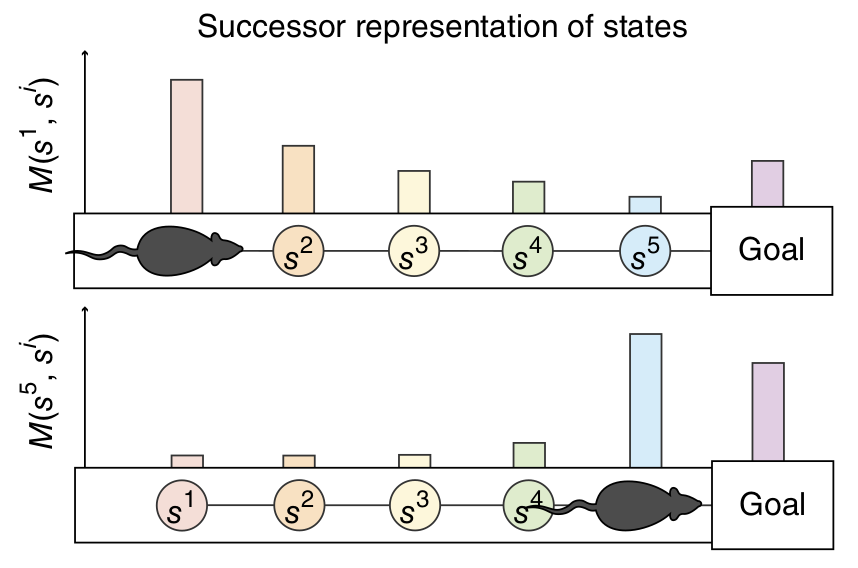
\includegraphics[height=0.6\textheight]{Bilder/Beispiel_SR_Zeile.png}
	\end{figure}
	\notsoimportant{Superscript means index not power; image taken from~\cite{StBoGe17HPM}}
\mynote{
    \begin{itemize}
        \item[ü] It is possible to interpret the rows and columns of the SR, which we will do now. Before we analyze the image, some information about the context in which the values where taken
        \item[i] The cognitive rooms consists of $ 6 $ states in total
        \item[i] The policy has to actions: going one step or pausing
        \item[i] The upper half depicts the first row of matrix $ M $ and implies the following: Due to the ``stay or pause''-policy the probability for the states $ s^1, \ s^2 $ is the largest.
        \item[i] The same goes for the lower half with state $ s^5 $ and \texttt{goal}
    \end{itemize}
}
\end{frame}

% === Successor Representation: Column ===================================

%\begin{frame}{Successor Representation}{Example 2/2 of interpreting a SR matrix $ M $}
%% TODO Bildquelle angeben
%    \begin{itemize}
%    	\item<+-> Column $ j $: High value in component $ i $, e.g. $ s^4 $, means state $ j $ is visited regularly after starting at state $ i $
%    \end{itemize}
%    \begin{figure}[c]
%		\centering
%			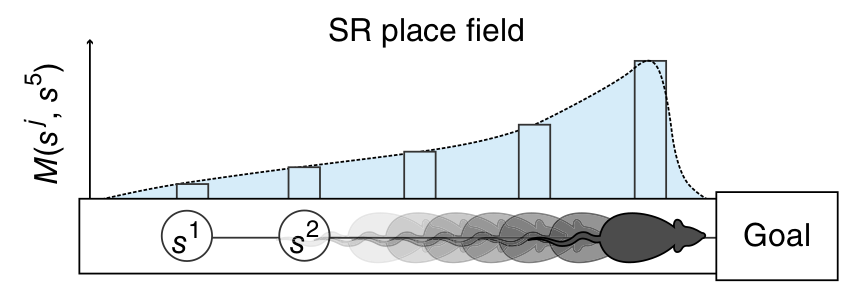
\includegraphics{Bilder/Beispiel_SR_Spalte.png}
%	\end{figure}
%    \notsoimportant{image taken from~\cite{StBoGe17HPM}}
%% -- NOTIZEN ------------------------------------
%\mynote{
%\begin{itemize}
%    \item[ü] Inspection now the column of the matrix $ M_a $
%	\item We can recognize the development of the policy: The more often the rat/mice goes to the right, the more likely it becomes reaching state $ s^4 $ or $ s^5 $ and the that pausing in $ s^5 $ is the most plausible.
%\end{itemize}
%}
%\end{frame}

% === Metric for quantifying the results ===================================

%\begin{frame}
%\frametitle{Metric for quantifying the results}
%	\begin{itemize}
%		\item<+-> To evaluate the results, we will use the following metric on the space $ \mathcal{P} $ of $ n \times m $-probability matrices:
%		\begin{equation}
%			d_A \colon \mathcal{P} \to [0,1], \qquad L \mapsto \frac{1}{\sqrt{2 \cdot n}}\Vert A - L \Vert_2
%			\text{,}
%		\end{equation}
%		with $ A \in \mathcal{P} $.
%		\item<+-> $ d_A $ was designed by me to map $ L $ close to $ 0 $ if it is similar to $ A $ and to $ 1 $ if both don't share plenty of features.
%		\item<+-> In our cases the ground truth will play the role of $ A $
%		\item<+-> \hint{Disclaimer: The metric was developed to compare the results with each other not to classify results independently.}
%%		\begin{itemize}
%%			\item<+-> $ d_A(X) = 0.15 $ and $ d_A(Y) = 0.78 \Longrightarrow X $ is closer to $ A $ than $ Y $ but not ``$ X $ is a good fit of $ A $''
%%		\end{itemize}
%	\end{itemize}
%% --------------------------------------
%\mynote{
%	\begin{itemize}
%		\item Because we are dealing with high dimensional sparse matrices, we can't just look at them to recognize whether leaning worked or not. Furthermore visuals are subjective, hence we need an objective measure to assess the results. METRIK VORLESEN
%		\item $ d_A $ was designed by me to map $ L $ close to $ 0 $ if it is similar to $ A $ and to $ 1 $ if both don't share plenty of features.
%		\item In our cases the ground truth will play the role $ A $
%		\item Last but not least a disclaimer: \hint{The metric was developed to compare the results with each other not to classify results independently.}; That means a low value not necessarily means that learning was successful. The results of the metric make sense in comparison to other mappings of $ d_A $. 
%	\end{itemize}
%}
%\end{frame}